% TODO: follow Beamer Users' Guide!

% Settings
\documentclass[11pt]{beamer}

% packages
\usepackage[utf8]{inputenc}
\usepackage{amsmath}
\usepackage{amsfonts}
\usepackage{array}
\usepackage{booktabs}
\usepackage{bxdpx-beamer}
\usepackage{colortbl}
\usepackage{dcolumn}
\usepackage{floatrow}
\usepackage{geometry}
\usepackage{graphicx}
\usepackage{hyperref}
\usepackage{multirow}
\usepackage{natbib}
\usepackage[normalem]{ulem}
\usepackage{pdflscape}
\usepackage{rotating}
\usepackage{setspace}
\usepackage{siunitx}
\usepackage{subfigure}
\usepackage{tabularx}
\usepackage{tcolorbox}
\usepackage{threeparttable}
\usepackage{ulem}
\usepackage{wrapfig}
\usepackage{xcolor}
\tcbuselibrary{fitting}


\PassOptionsToPackage{height=1.4cm}{beamerouterthemesidebar}  % custom header size
\usetheme{PaloAlto}  
\usecolortheme{default}
\usefonttheme{structurebold}
% \setbeamercovered{transparent}
\setbeamertemplate{caption}[numbered]
\setbeamertemplate{footline}[frame number]
\newcommand{\indicatewidth}[1]{\thickhrulefill{#1}\thickhrulefill}
\newcommand{\thickhrulefill}{\leavevmode\leaders\hrule depth-1.2pt height 3.2pt\hfill\kern0pt}
\newlength{\mytotalwidth}
\mytotalwidth=\dimexpr\linewidth-5mm
\newlength{\mycolumnwidth}
\mycolumnwidth=\dimexpr\mytotalwidth-5mm

\renewcommand<>{\sout}[1]{
  \temporal#2{\invisible{#1}}{#1}{\beameroriginal{\sout}{#1}}
}

%------------------------------------------------------------
% This block of code defines the information to appear in the
% Contents of the title page
\title[Youth and Party Nomination]{Youth Underrepresentation and \\ Parties' Nomination Strategy in \\ Mixed-Member Systems}
\author[Dai Sasaki (UTokyo)]{ \href{https://dxxsxsxkx.github.io/}{Dai Sasaki}\inst{1}}
\institute[UTokyo]
{
    \inst{1}
    Graduate Schools for Law and Politics \\
    The University of Tokyo
}
\date[JSQPS 2024 Summer]{JSQPS Summer Meeting 2024 (Jul 6, 2024)}

\begin{document}

% Title
\frame{\titlepage}

\section{Overview}

% Overview
\begin{frame}

\frametitle{Puzzle: Youth Representation in Japan}
	\begin{itemize}
		\item U40 MPs: 6\% in 2023
		\begin{itemize}
			\item Mixed-member system (SMD + PR) in the lower house
		\end{itemize}
		\item PR should promote youth representation, but...
		\begin{itemize}
			\item Winners' age: 53.7 (SMD) vs. 53.0 (PR)
		\end{itemize}
	\end{itemize}

	\begin{figure}[H]
		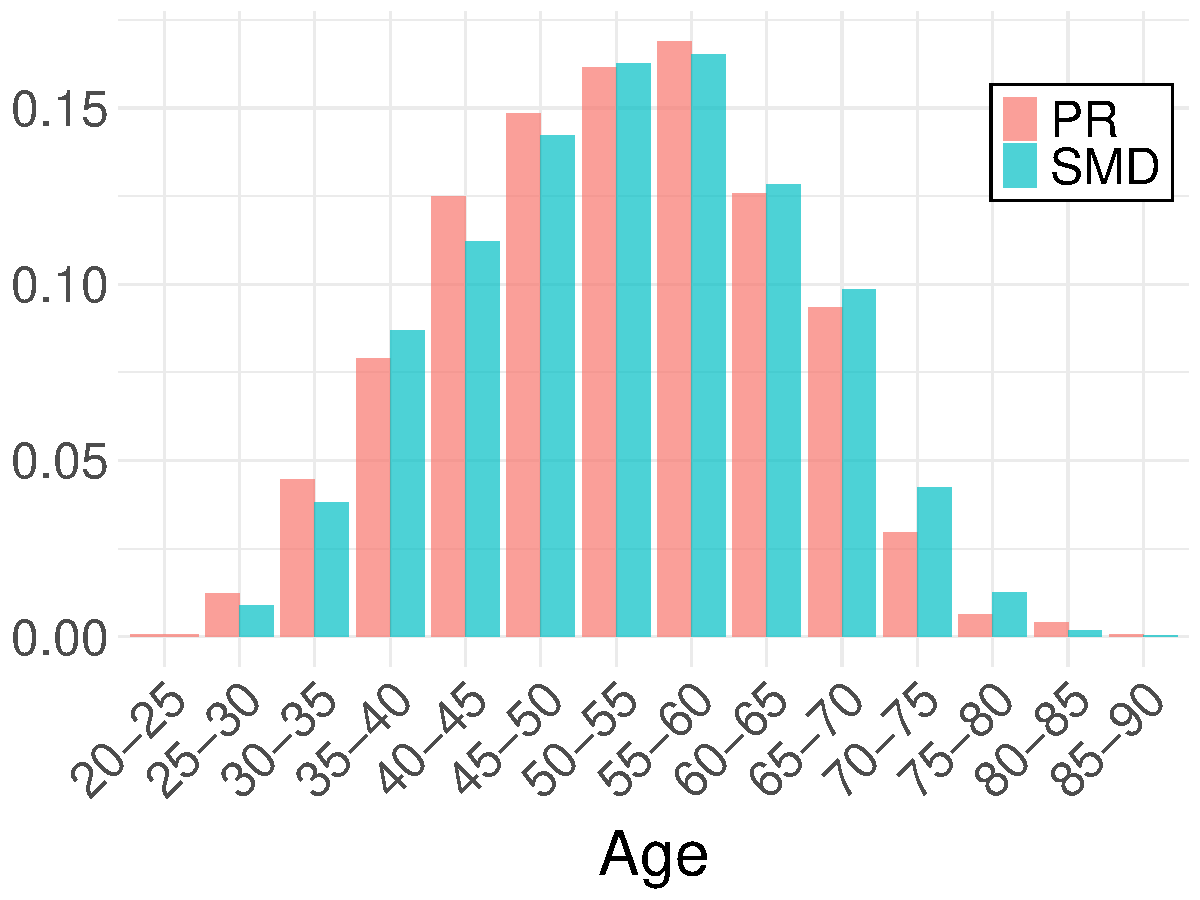
\includegraphics[width=180pt]{../figure/slide/age_smd_vs_pr_winners.pdf} 
	\end{figure}

\end{frame}


\begin{frame}{Today's Talk}

\begin{itemize}
	\item \textbf{RQ.} Why does the PR tier in Japan's mixed member system underrepresent young people? 
	
	\item Explain how \alert{dual listing} gives parties incentives to give their senior members and incumbents \alert{``second chances"}, preventing new candidates' entries via the PR tier. 
	
	\item Present evidence from the House of Representatives elections, 1996 - 2017. 
		
	\item Discuss implications for comparative politics. 
	
\end{itemize}

\end{frame}


% Theory
\section{Theory}

\begin{frame}  %TODO: fix, fewer words
	\frametitle{Do Electoral Systems Affect Youth Underrepresentation?}
	
	\begin{itemize}
		\item PR promotes minority representation \citep{norris_electoral_2004}
		
		\begin{itemize}
			\item Collective evaluation of party lists
			
			\item Party incentives to represent various cleavages
		\end{itemize}
		
		\item More young MPs under PR (e.g., \citet{joshi2013representation})
		
		\begin{itemize}
			\item Cross-national studies
			
			\item Does not answer "how"
		\end{itemize}
	
		\item We don't know what happens in mixed-member systems. 
		
		\begin{itemize}
			\item ``Best of the both worlds"? 
			
			\item PR $>$ MM $>$ majoritarian? 
		\end{itemize}
	\end{itemize}
	
\end{frame}

\begin{frame}<1>[label=jpmixed]  %TODO: fix
	\frametitle{Japan's Mixed-member System}
	\begin{itemize}  
		\item Mixed-member majoritarian (MMM)
		
		\begin{itemize}
			\item SMDs (SNTV) + PR blocks (closed lists)
						
		\end{itemize}
		
		\item \alert{Dual listing}  
		
		\begin{itemize}  
			
			\item Can nominate candidates simultaneously in the two tiers
			
			\item Can give any of dual-listed candidates the same rank within a list 
			
			\item ``Best-loser" rule to decide winners among equally-ranked candidates
			
			\item<alert@1> Very common
			
			\item A source of ``contamination effects" (e.g., \citet{ferrara_mixed_2005})? 
		\end{itemize}
	\end{itemize}
\end{frame}

\begin{frame}{Dual Listing is Very Common}
	\begin{figure}[H]
		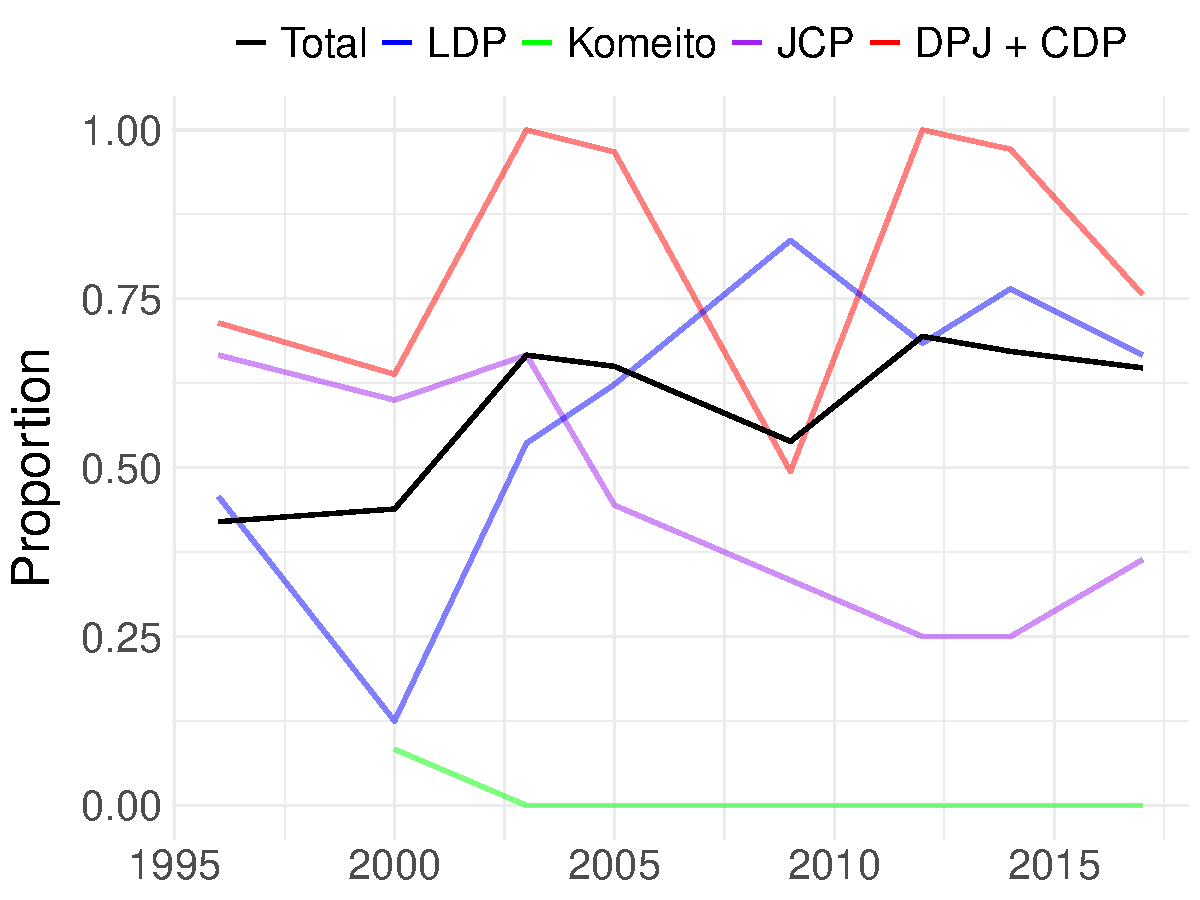
\includegraphics[width = 0.8\textwidth]{../figure/slide/dual_nomination.pdf}
		\caption{Proportion of Dual-Listed Winners}
	\end{figure}
\end{frame}

\againframe{jpmixed}

\begin{frame}  %TODO: fix
	\label{Main claim}
	\frametitle{Dual Listings Would Exacerbate Youth Representation}  
	\begin{alertblock}{Claim}  % main claim
        		Dual listing 
		\begin{itemize}
			\item incentivizes parties to give second chaces to senior candidates / incumbents
			\item prevents younger candidates' entry via PR tier. 
		\end{itemize}
    	\end{alertblock}
	
	Parties would dual-list their senior members when possible.  
	\begin{itemize}
		\item Post-election goals, e.g., policies. 
		\item Coalition formation. 
		\item Distribution of ministerial posts. 
		\item Legislation. 
	\end{itemize}
		
	Less frequent turnover $\rightarrow$ youth underrepresentation

\end{frame}

\begin{frame}{Hypotheses}  
\begin{itemize}
	\item List rank
	\begin{enumerate}
		\item[1.] Dual-listed candidates are ranked higher. 
		
		\item[2.] Incumbents are ranked higher. 
		
		\item[3.] Senior candidates are ranked higher. 
		
	\end{enumerate}
		
	\item Dual listing
	\begin{enumerate}	
		\item[4.] Incumbents are more likely to be dual-listed. 
		
		\item[5.] Senior candidates are more likely to be dual-listed.
	\end{enumerate}
\end{itemize}
\end{frame}

\section{Data and Method}

\begin{frame}
	\frametitle{Data}
	Data: the Reed-Smith JHRED \citep{reedsmith2018}
	\begin{itemize}
		\item PR candidates
				
		\item 1996, 2000, 2003, 2005, 2009, 2012, 2014, 2017
	\end{itemize}
			
\end{frame}

\begin{frame}
	\frametitle{Empirical Strategy}		
	H1 - 3: Negative binomial models
	\begin{itemize}
		\item DV: candidate $i$'s list rank (minus 1)  % to facilitate interpretation (how many candidates are above?)
			
		\item IV: candidate $i$'s dual-listing status; N of past wins; incumbency status
			
		\item Controls: female dummy, District magnitude, year and party FEs
			
	\end{itemize}
	
	H4 - 5: Logistic models
	\begin{itemize}
		\item DV: candidate $i$'s dual-listing status 
			
		\item IV: candidate $i$'s N of past wins; incumbency status
			
		\item Controls: female dummy, District magnitude, year and party FEs
			
	\end{itemize}
			
\end{frame}


\section{Result}

\begin{frame}  % H1
	\frametitle{H1: Dual-Listed Candidates Ranked Higher}
	
	\begin{itemize}
		\item Male, LDP, Tokyo Block ($M = 20$), 2012
	\end{itemize}
	
	\begin{figure}[H]
	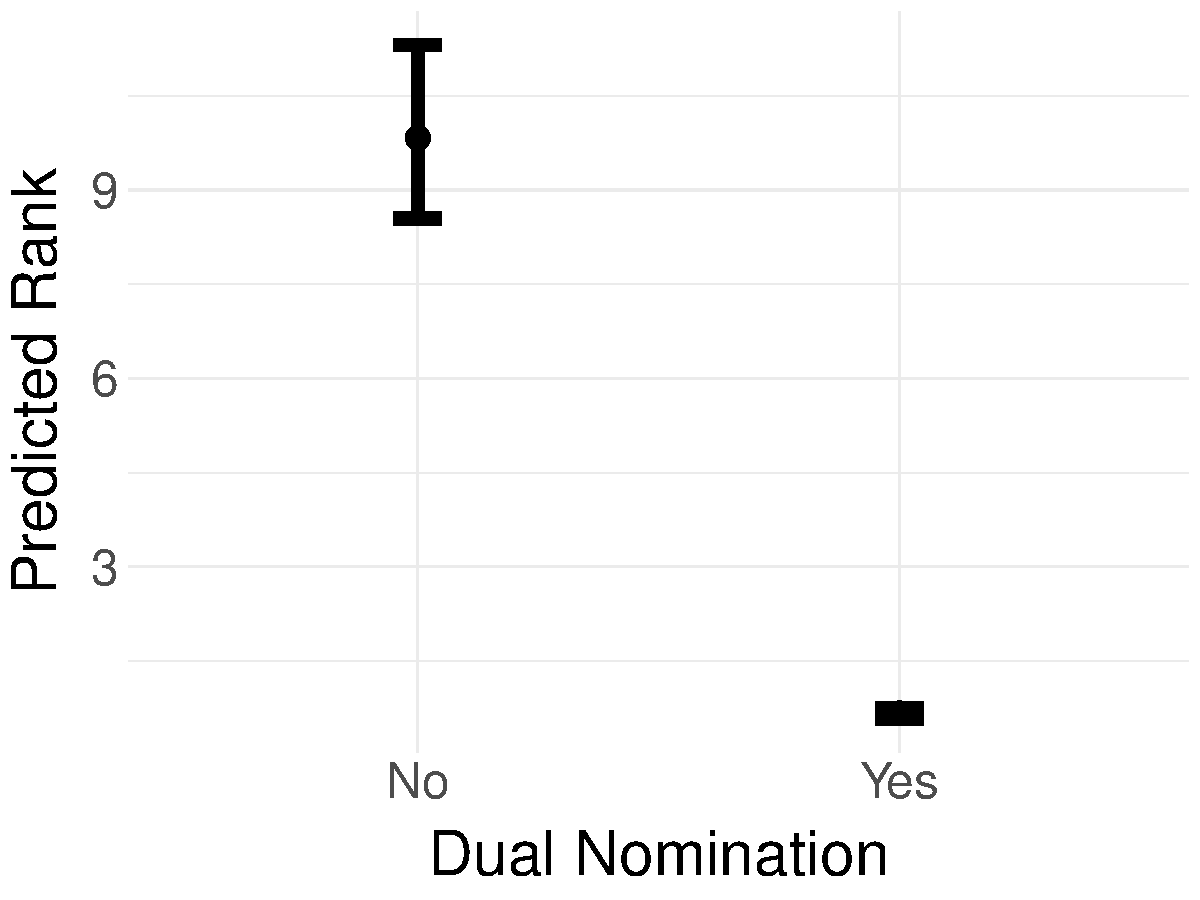
\includegraphics[width = 0.7 \textwidth]{../figure/slide/h1_dual_nomination.pdf}
    	\end{figure}

\end{frame}

\begin{frame}  % H2
	\frametitle{H2: Incumbents Ranked Higher}
	
	\begin{itemize}
		\item Male, LDP, Tokyo Block ($M = 20$), 2012
	\end{itemize}
	
	\begin{figure}[H]
	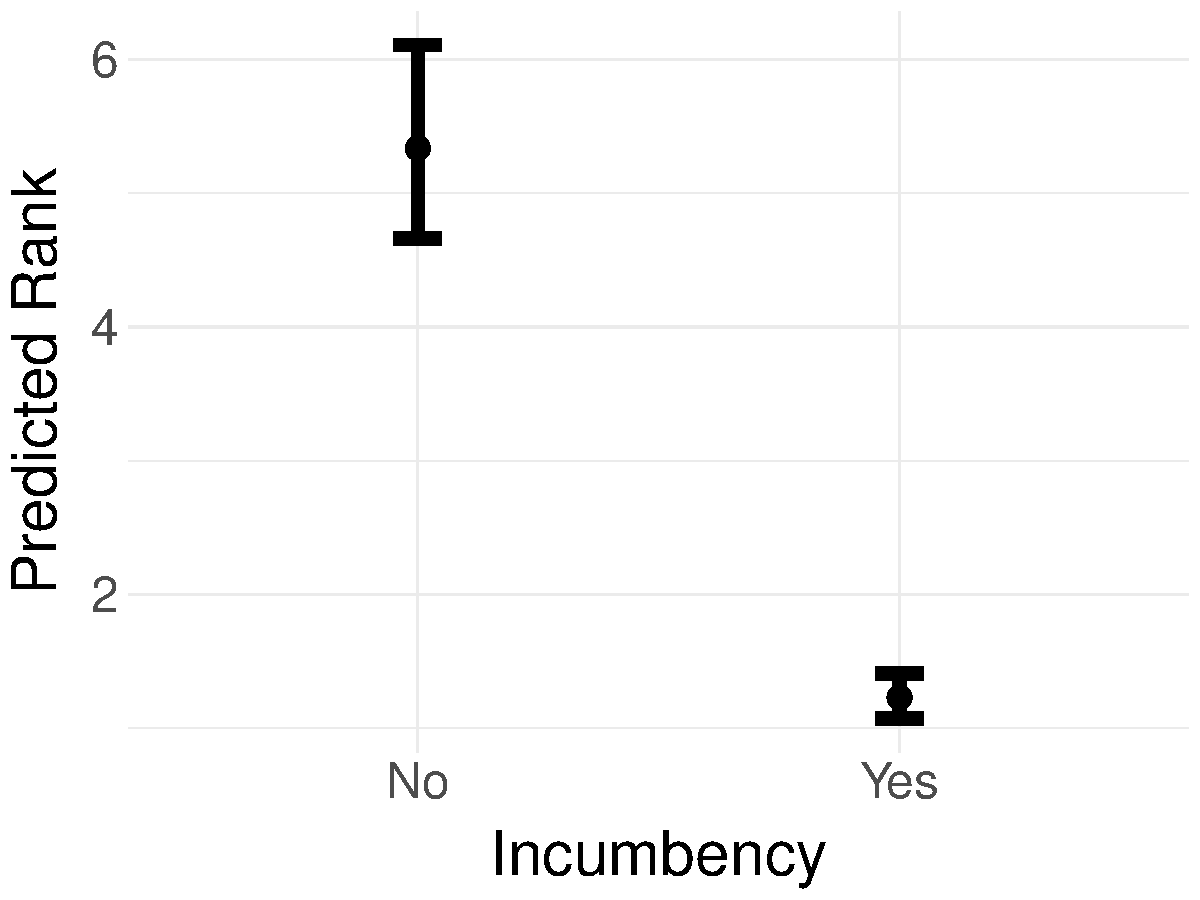
\includegraphics[width = 0.7 \textwidth]{../figure/slide/h2_incumbency.pdf}
    	\end{figure}

\end{frame}

\begin{frame}  % H3
	\frametitle{H3: Senior Candidates Ranked Higher}
	
	\begin{itemize}
		\item Male, LDP, Tokyo Block ($M = 20$), 2012
	\end{itemize}
	
	\begin{figure}[H]
	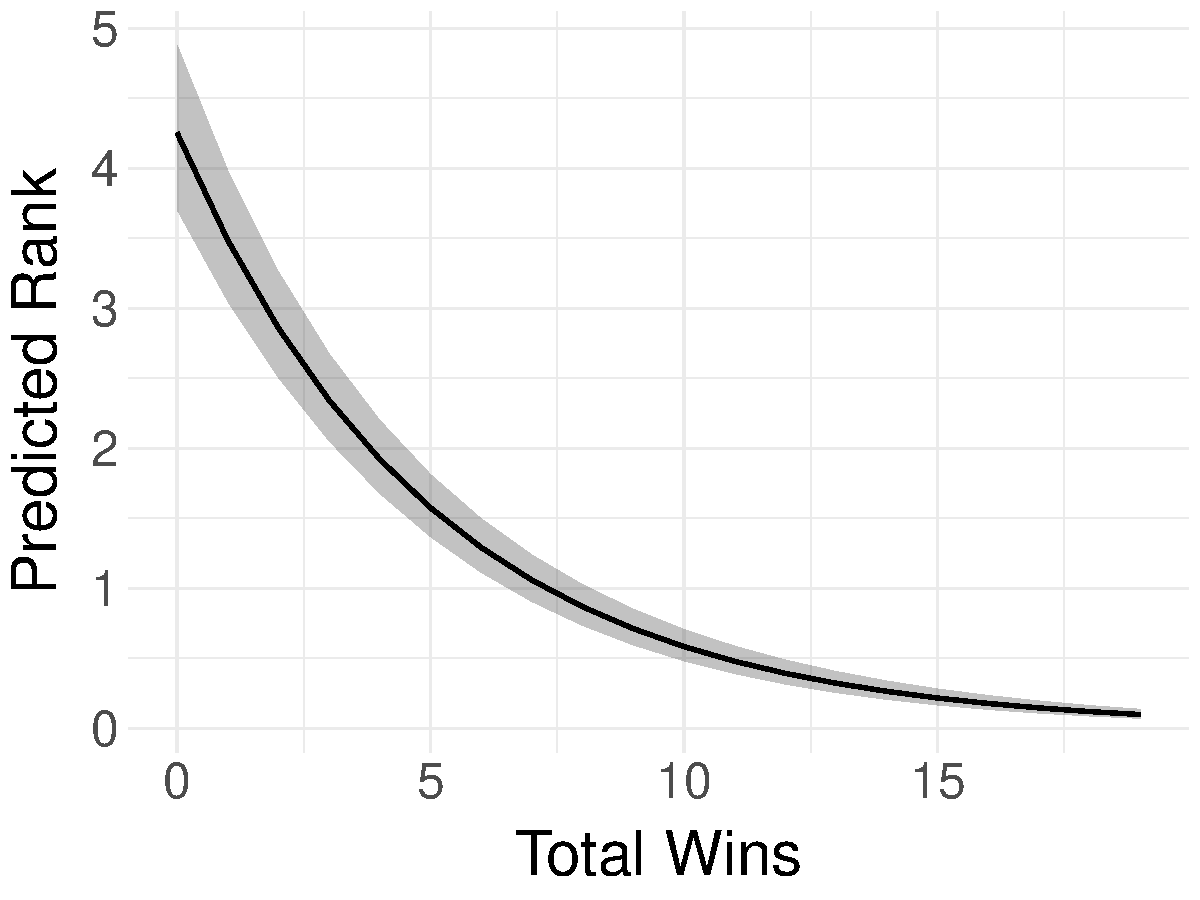
\includegraphics[width = 0.7 \textwidth]{../figure/slide/h3_total_wins.pdf}
    	\end{figure}

\end{frame}

\begin{frame}  % H4 
	\frametitle{H4: Incumbents More Likely to be Dual-Listed}
	
	\begin{itemize}
		\item Male, LDP, Tokyo Block ($M = 20$), 2012
	\end{itemize}
	
	\begin{figure}[H]
	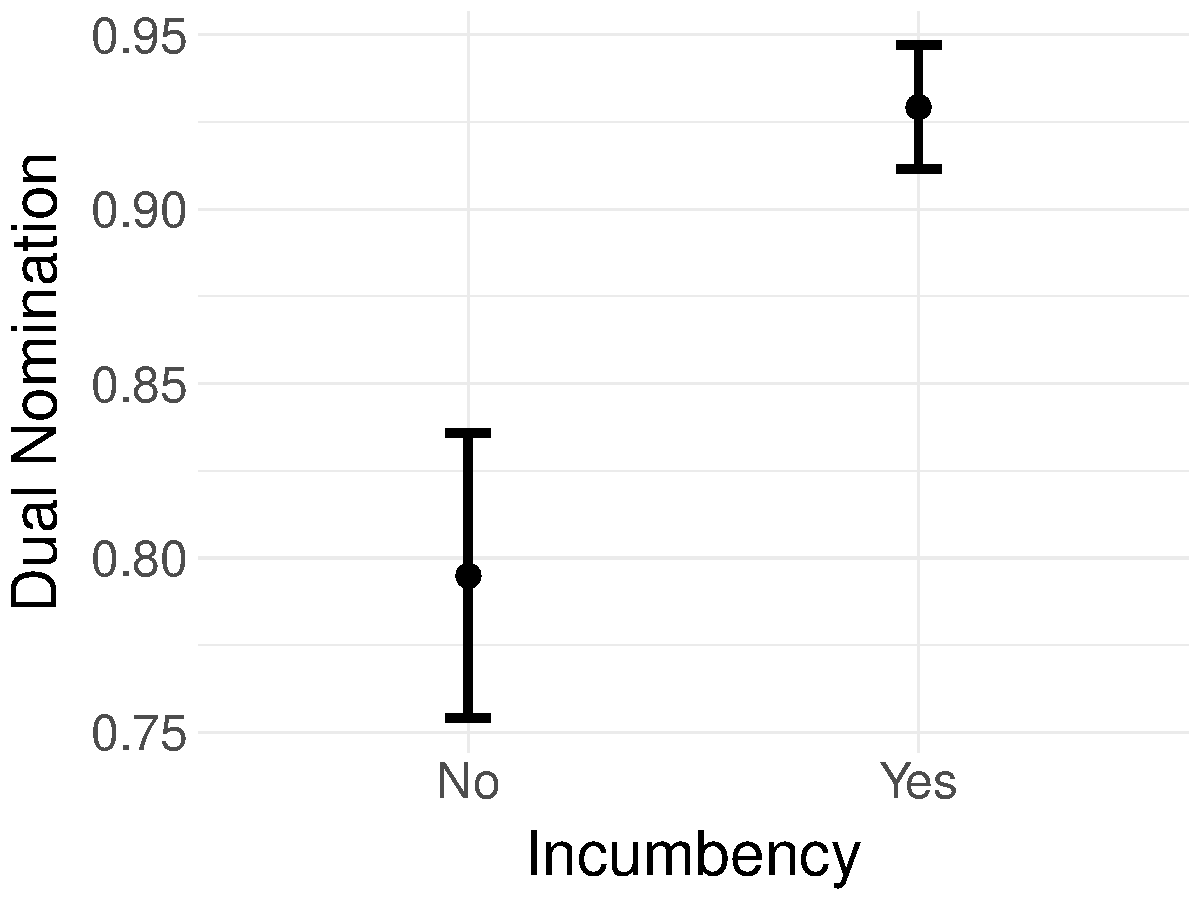
\includegraphics[width = 0.7 \textwidth]{../figure/slide/h4_incumbency.pdf}
    	\end{figure}

\end{frame}

\begin{frame}  % H5 
	\frametitle{H5: Senior Candidates More Likely to be Dual-Listed}
	
	\begin{itemize}
		\item Male, LDP, Tokyo Block ($M = 20$), 2012
	\end{itemize}
	
	\begin{figure}[H]
	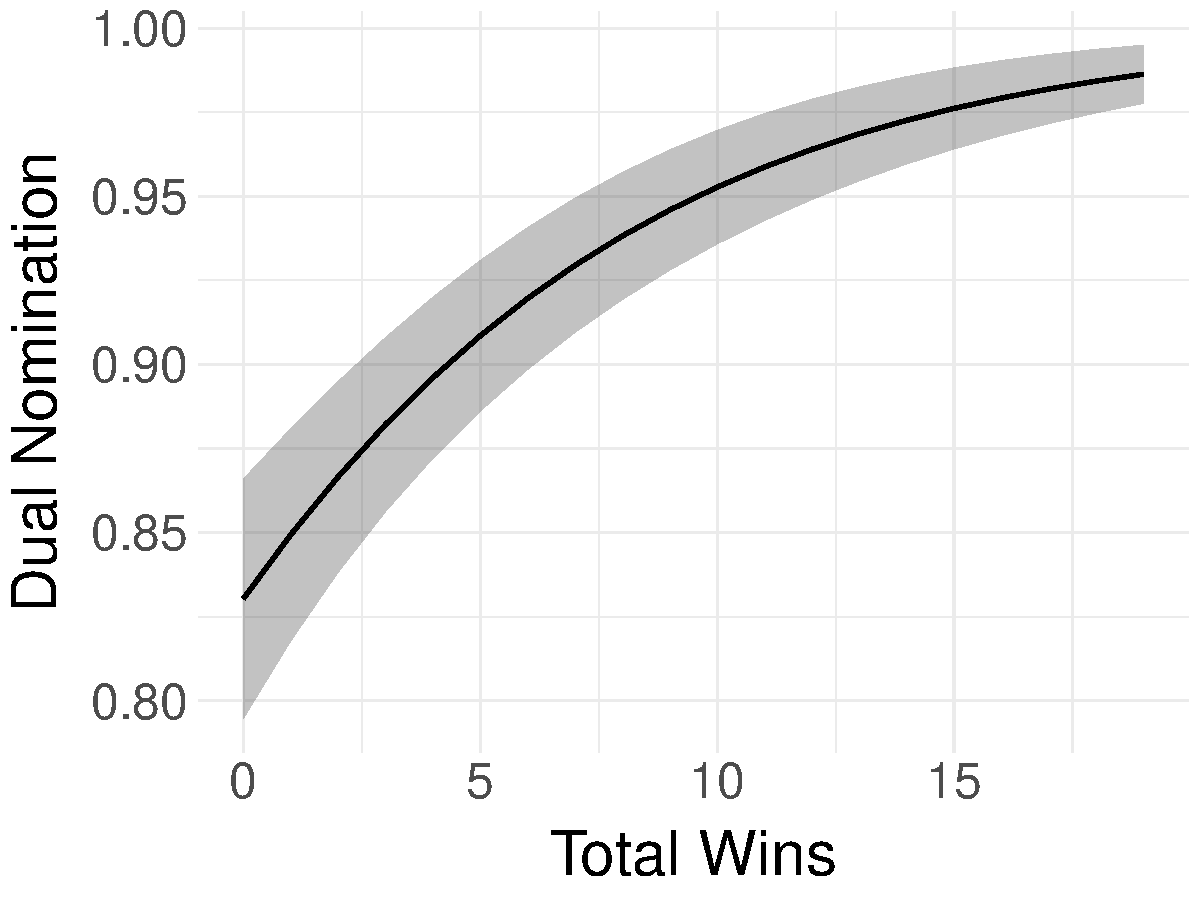
\includegraphics[width = 0.7 \textwidth]{../figure/slide/h5_total_wins.pdf}
    	\end{figure}
	
\end{frame}

\section{Discussion}

\begin{frame}
	\frametitle{Findings}
	
	\begin{alertblock}{Claim}  % main claim
        		Dual listing 
		\begin{itemize}
			\item incentivizes parties to give second chaces to senior candidates / incumbents
			\item prevents younger candidates' entry via PR tier. 
		\end{itemize}
    	\end{alertblock}

	
	\begin{enumerate}
		\item Dual-Listed Candidates are ranked higher. 
		
		\item Incumbents are ranked higher. 
		
		\item Senior candidates are ranked higher. 
		
		\item Incumbents are more likely to be dual-listed. 
		
		\item Senior candidates are more likely to be dual-listed. 
	\end{enumerate}

\end{frame}

\begin{frame}
	\frametitle{What If Dual Listing Had Not Been Allowed?}
	
	\begin{itemize}
		\item Parties have incentives to nominate young candidates in PR. 
		\begin{itemize}
			\item Competing incentive to give out insurances under dual listing
		\end{itemize}
	
		\item Parties would have nominated new candidates instead of incumbents / senior members. 
		
		\item \alert{New candidates are younger than other candidates / MPs.}
		
		\item Youth underrepresentation would have been mitigated. 
	\end{itemize}
	
\end{frame}

\begin{frame}
	\frametitle{What If Dual Listing Had Not Been Allowed?}
	
	\begin{itemize}
		\item New candidates are much younger than the average.
	\end{itemize}
	
	\begin{table}[H]
	\begin{tabular}{l  c c c c}
		Year & All & Novice \\
		\hline 
		1996 & 52.3 & 46.9 \\
		2000 & 52.4 & 46.8 \\
		2003 & 51.0 & 44.6 \\
		2005 & 50.6 & 44.9 \\
		2009 & 52.0 & 48.2 \\
		2012 & 49.6 & 44.5 \\
		2014 & 51.6 & 48.7 \\
		2017 & 52.0 & 48.7 \\
		\hline
	\end{tabular}
	\caption{Age Comparison: PR Candidates}	
	\end{table}
\end{frame}

\begin{frame}
	\frametitle{What If Dual Listing Had Not Been Allowed?}
	
	\begin{itemize}
		\item Parties have incentives to nominate young candidates in PR. 
		\begin{itemize}
			\item Competing incentive to give out insurances under dual listing
		\end{itemize}
	
		\item Parties would have nominated new candidates instead of incumbents / senior members. 
		
		\item New candidates are younger than other candidates / MPs.
		
		\item Youth underrepresentation would have been mitigated. 
	\end{itemize}
	
\end{frame}

\begin{frame}{Implications and What's Next}
	
\begin{itemize}
	\item Implications: 
	\begin{enumerate}  
		\item Contamination effects in MM systems reduce representational advantages of PR systems. 
		
		\item In terms of minority representation, MM systems are not in the middle between majoritarian and PR systems. 
		
		\item A potential mechanism of youth underrepresentation:  \\ Electoral system $\rightarrow$ party incentives $\rightarrow$ youth representation  
		
	\end{enumerate}
	
	\item What's next
	\begin{itemize}
		\item More elaborated theory
		\item What about MM systems in other contexts? 
		\item What about other minority groups, e.g., women? 
	\end{itemize}
	
	\item Limitation: counterfactuals
	\begin{itemize}
		\item Path-dependence of nomination strategies
		\item Identities of counterfactual nominees
	\end{itemize}

	
\end{itemize}
	
\end{frame}


\begin{frame}{References}  
    \scriptsize
    \beamertemplatetextbibitems
    \bibliography{../Reference.bib}
    \bibliographystyle{apalike}
\end{frame}

\appendix

\begin{frame}
\frametitle{Motivation: Youth Underrepresentation}

	\begin{itemize} 
		\item Youth underrepresentation in many democracies. Why? 
	\end{itemize}
	
	\begin{figure}[H]
		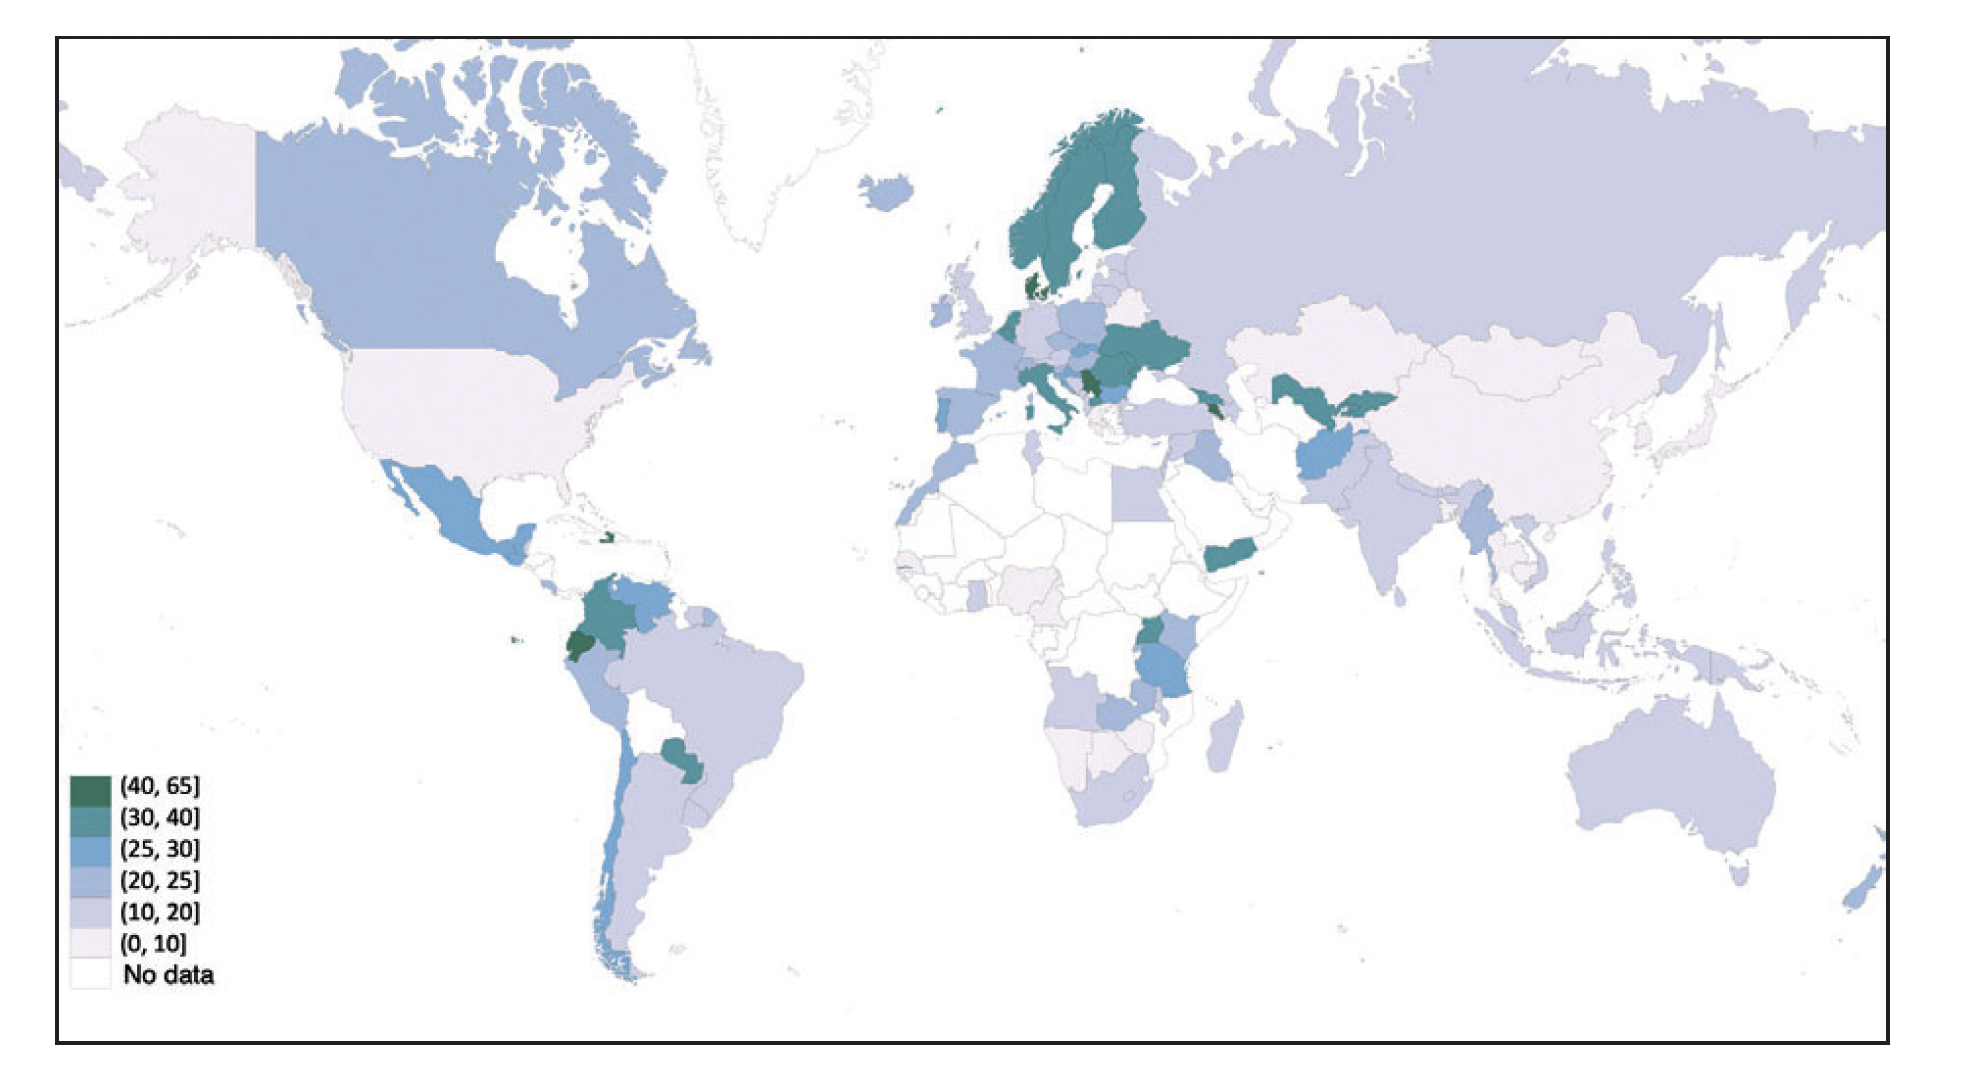
\includegraphics[width = 0.9\textwidth]{../figure/stockemer_sandstrom.png}
		\caption{Proportion of U40 MPs. From \citet[p.47]{stockemer_youth_2022}.}
	\end{figure}

\end{frame}

% Youth underrepresentation in advanced democracies
\begin{frame}{Youth Underrepresentation in G7 Countries}  %TODO: それぞれのケースについて選挙制度とかを把握しておく. 


\begin{table}[H]
% latex table generated in R 4.1.0 by xtable 1.8-4 package
% NOTE: manually modified on 27 Nov 2023. 
% Sat Jul  8 06:31:47 2023
\begin{tabular}{lccccc}
\toprule
Country & Eligibility & Average & \% U30 & \% U40 & \% U45 \\ 
\midrule
Canada & 18 & 50 & 1.95 & 16.88 & 30.19 \\ 
France & 18 & 49 & 4.85 & 26.52 & 37.95 \\ 
Germany & 18 & 47 & 8.83 & 28.94 & 41.98 \\ 
Italy & 25 & 49 & 1.25 & 16.25 & 35 \\ 
Japan & 25 & 55 & 0.22 & 6.02 & 17.2 \\ 
UK & 18 & 51 & 3.69 & 21.69 & 34 \\ 
USA & 25 & 57 & 0.46 & 10.42 & 20.14 \\ 
\bottomrule
\end{tabular}

\caption{\textit{Source.} \citet{ipu2023}.}
\end{table}

\end{frame}

% Joshi(2013)

\begin{frame}

\frametitle{Puzzle: Youth Representation in Japan}

	\begin{columns}[totalwidth=\mytotalwidth]
     		\begin{column}[T]{0.5\mycolumnwidth}
			\centering
        			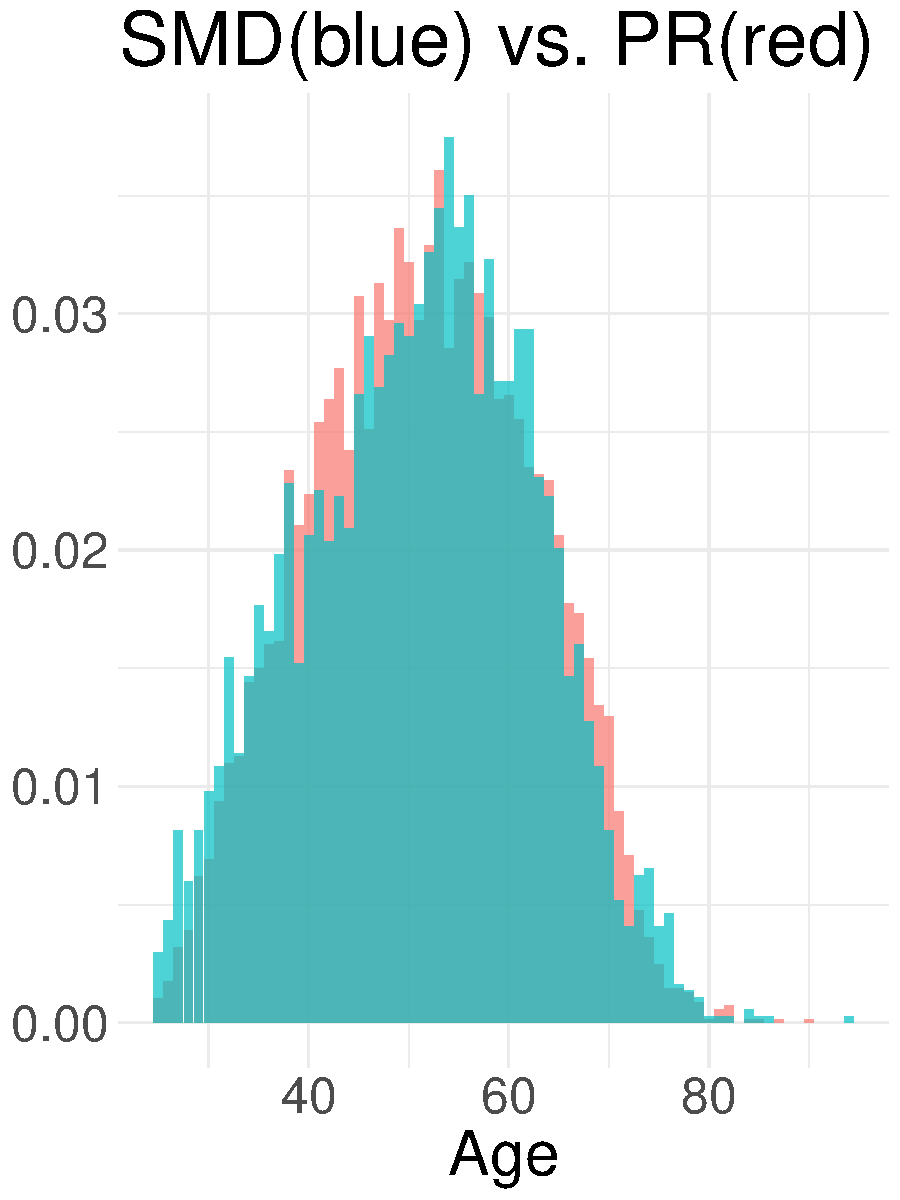
\includegraphics[width=120pt]{../figure/slide/age_smd_vs_pr.pdf}
      		\end{column}
      		\begin{column}[T]{0.5\mycolumnwidth}
		\begin{itemize}
			\item Mixed-Member system: SMD + PR
			\item PR should promote youth representation, but...
			\item \alert{Candidates}' mean age: 
			\begin{itemize}
				\item SMD: 51.0
				\item PR: 51.4
			\end{itemize}
		\end{itemize}
      		\end{column}
    	\end{columns}

\end{frame}

\begin{frame}
	\frametitle{No Evidence that Pure-PR Candidates are Younger}
	
    	\begin{columns}[totalwidth=\mytotalwidth]
     		\begin{column}[T]{0.5\mycolumnwidth}
			\centering
        			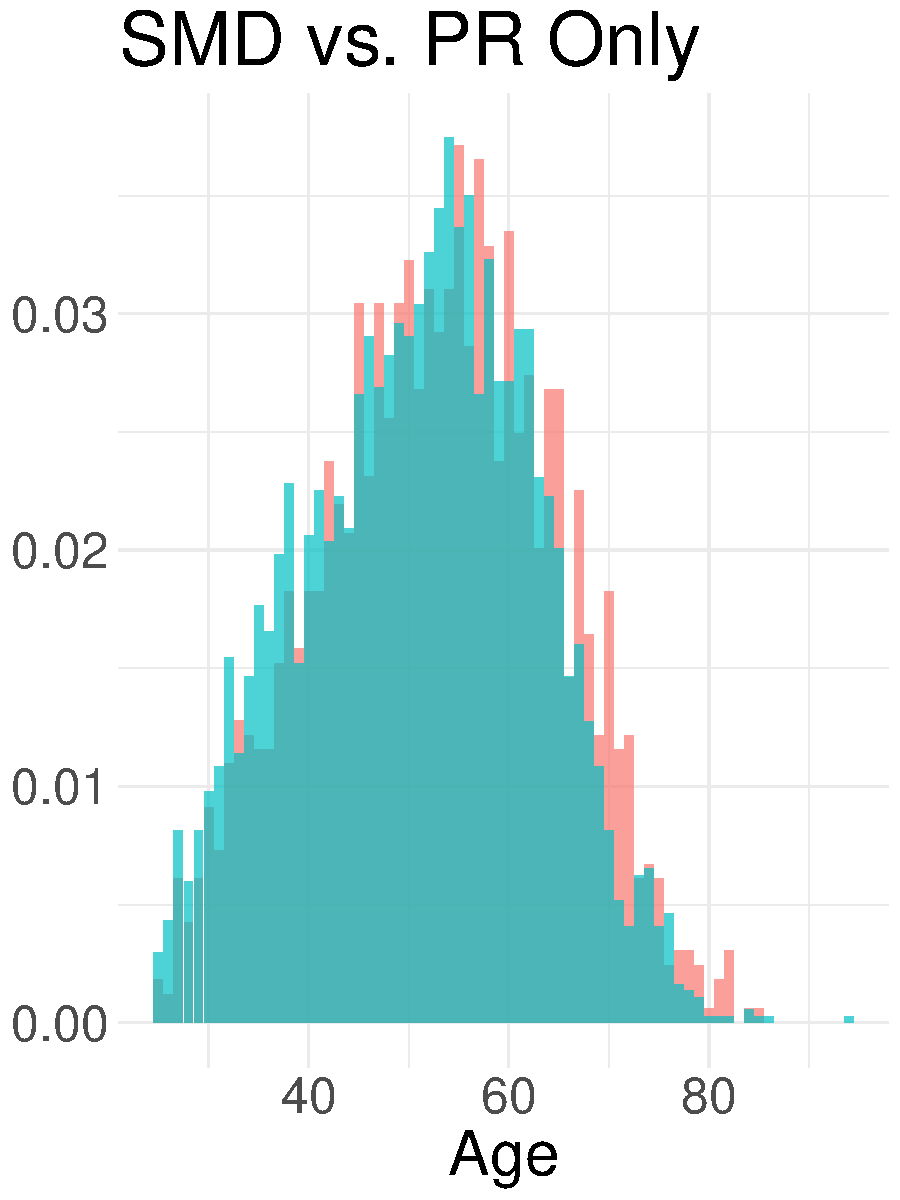
\includegraphics[width=120pt]{../figure/slide/age_smd_vs_pr_only.pdf}
      		\end{column}
      		\begin{column}[T]{0.5\mycolumnwidth}
		Mean age: 
		\begin{itemize}
			\item SMD: 51.0
			\item PR: 52.8
		\end{itemize}
      		\end{column}
    	\end{columns}

\end{frame}

\begin{frame}
	\frametitle{What If Dual Listing Had Not Been Allowed?}
	
	\begin{itemize}
		\item New candidates are younger across the two tiers. 
	\end{itemize}
	
	\begin{table}[H]
	\begin{tabular}{l  c c c c}
		Year & Age (all) & Age (novice)\\
		\hline 
		1996 & 51.1 & 47.5 \\
		2000 & 51.6 & 47.7 \\
		2003 & 51.1 & 47.0 \\
		2005 & 50.6 & 46.4 \\
		2009 & 50.9 & 47.2 \\
		2012 & 50.4 & 47.0 \\
		2014 & 52.2 & 49.9 \\
		2017 & 52.8 & 49.4 \\
		\hline
	\end{tabular}
	\caption{Age Comparison: SMD + PR Candidates}	
	\end{table}

\end{frame}

\end{document}